\chapter{Introduction}

\section{The Case for New Solar Absorber Materials for Photovoltaic Devices}

\subsection{Terawatt-Scale Energy Production from Renewable Resources}

It is now widely accepted that the world is heading towards a major energy crisis, where there will come a point that the current major sources of energy (namely fossil fuels) will be unable to meet increasing global demand for energy as they are not a limitless supply. Furthermore, there is the ever present worry of climate change due to increased carbon dioxide emissions caused by such types of energy generation. Renewable, low-carbon alternative energy sources are therefore clearly desirable. From purely an environmental sustainability perspective, it seems clear that fossil fuels should no longer be used and we should meet our energy needs solely from renewable, low-carbon energy sources. However, it is not only environmental sustainability that must be considered, we must also consider economical feasibility of solar power for large-scale projects. Germany is an example of a country making considerable efforts to increase the percentage of their energy supplied by solar power. On June 9 2014 Germany even generated over 50\% of its electricity demand from solar for the first time \cite{Germany_guardian_news}. Although on average the country is not able to produce such a large portion from solar power, with solar-generated power providing approximately 7.5\% of net electricity consumption in 2015 \cite{Germany_PV}. To facilitate the growth of the solar power capacity in Germany a number of schemes and financial incentives to encourage investment were introduced, such as feed-in tariffs (FiTs).
The German government first introduced FiTs in their Grid Feed-In Law (the Stromeinspeisegesetz), which came into force in 1991 \cite{Germany_Lang}. FiTs are intended to support new developments in renewable energy supply by providing investor certainty. They set the rate a utility company must pay for renewable generated energy and guarantee the provider of renewable energy a specific rate for a long period of time, typically fifteen to twenty years. As this cost is higher than fossil fuel based electricity, the higher price is then passed on to all customers of the utility company to spread out the higher costs so that buyers of renewable energy do not pay higher prices. In Germany, this has resulted in an increase of 6\% on the average electricity bill for users in a specific region \cite{Germany_Oregon}. The social implications of such a cost increase must also be considered in assessing the viability of a particular power source.

Solar energy is however a realistic candidate for replacing fossil fuels as a major supply of global energy. It is by far the largest source of energy available to us, as illustrated in figure \ref{global_energy}, and it is also the most widely geographically distributed \cite{inorg_pv}. The Sun supplies $3 \times 10^{24}$ J of energy to the Earth each year, which is $10^4$ times more than mankind's current annual energy consumption. In theory, this would require only 0.1\% of the Earth's surface to be covered in solar cells with a conversion efficiency of just 10\% to satisfy our current energy needs \cite{Gratzel}. Recent years have seen a rapid increase in the installed solar generation capacity, with the global grid-connected PV capacity growing from 1.3 GW in 2000 to 139 GW in 2014 \cite{pathways_129}, with approximately a doubling in the cumulative installed capacity every two years \cite{pathways}. Additionally, creative business models have spurred investment in residential solar systems \cite{MIT}. Great improvements in technology, price and performance have helped to facilitate this growth, but solar energy still only provides a minor fraction of the world's energy. In 2013 solar power only provided 0.87\% of the worlds electricity \cite{pathways_130}. Further advances are required to enable a dramatic increase in the contribution from solar power at socially acceptable costs \cite{MIT}. Ultimately, solar power-generation technologies must become cost-competitive with conventional fossil-fuel based power sources.\\

\begin{figure}[h!]
  \centering
    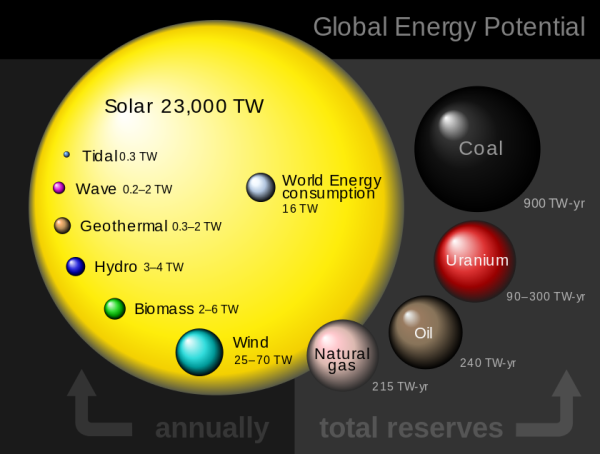
\includegraphics[width=0.75\textwidth]{figures/global_energy.png}
    \caption{Illustration of power available annually from various renewable energy resources, annual world energy consumption and total reserves of various non-renewable energy resources. Figure take from \citenum{global_energy_fig}.}
  \label{global_energy}
\end{figure}

\begin{figure}[h!]
  \centering
    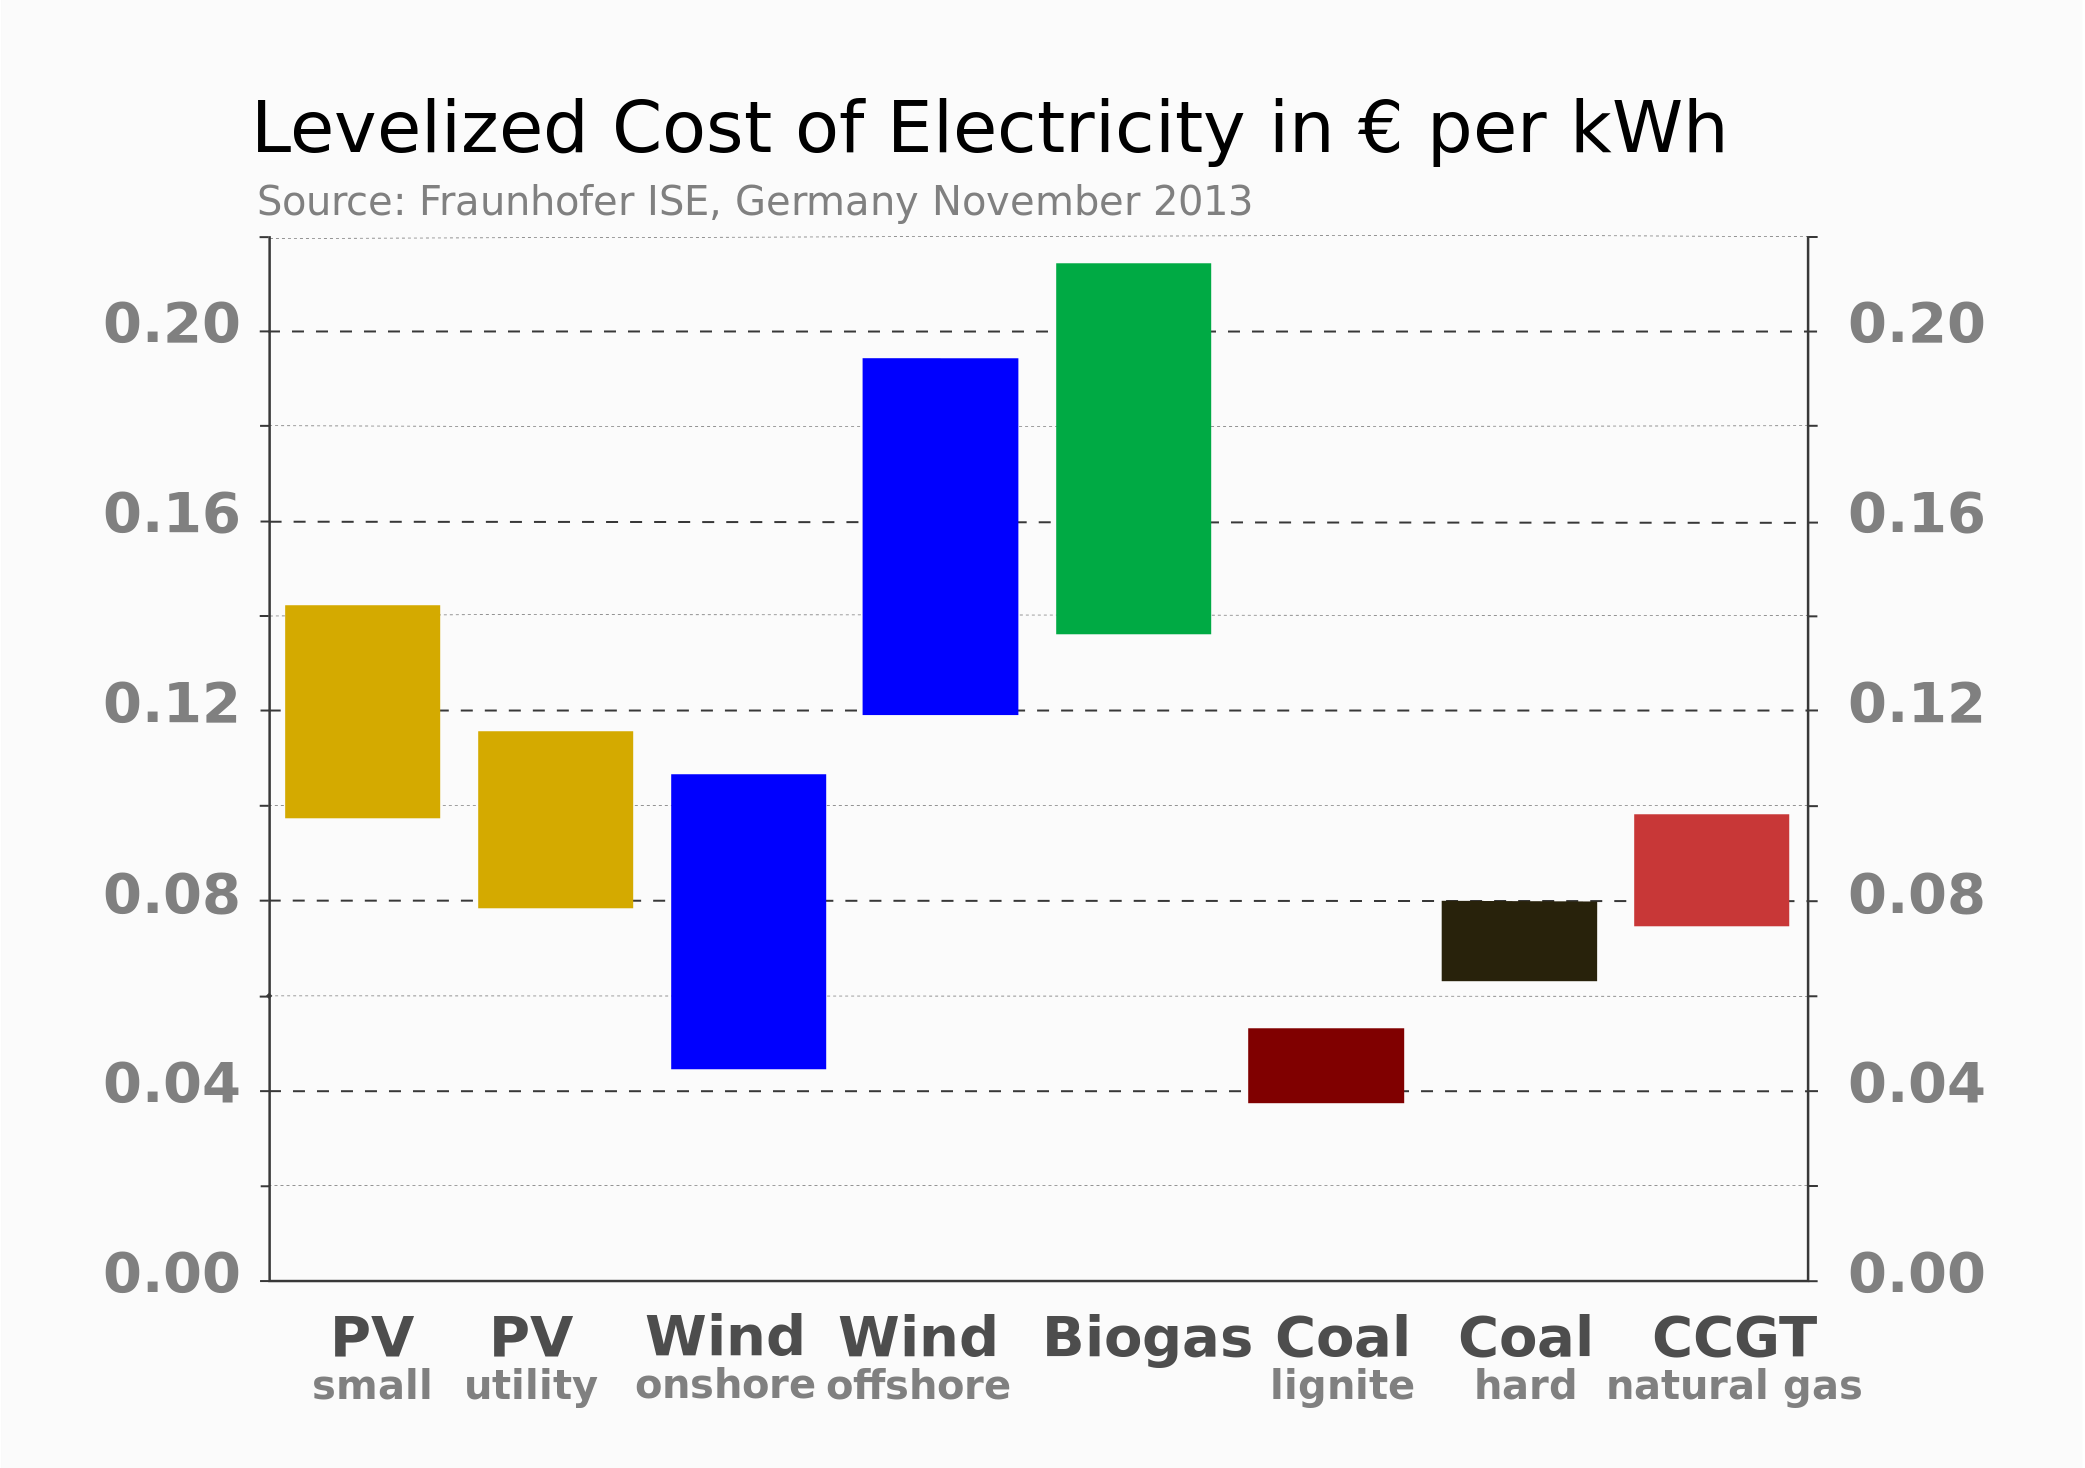
\includegraphics[width=0.8\textwidth]{figures/LCOE.png}
    \caption{Levelized cost of electricity (LCOE) of renewable energy technologies and conventional power plants at locations in Germany in 2013.  Specific investments are taken into account with a minimum and maximum value for each technology. Figure taken from reference \citenum{LCOE}.}
  \label{LCOE}
\end{figure}

Levelized cost of energy, or electricity, (LCOE) is a common way to assess how cost competitive renewable energy sources are with their non-renewable counterparts. LCOE allows for the measurement of the performance of different power generating technologies, which may have unequal lifetimes and differing capacities. It is calculated by summing all costs incurred during the lifetime of the technology and dividing this value by the units of energy produced during the lifetime, with units of energy expressed as dollars per kilowatt hour (\$/kWhr) \cite{LCOE2}. This measure is also used as the key selling point for a number of commercial solar cell manufacturers such as First Solar Inc., who market their product as being able to generate electricity at an average of \$0.63 per Watt as stated in their 2013  Annual Report \cite{first_solar}. Using the LCOE, comparisons of grid competitiveness for renewable energy sources can be made \cite{LCOE2}. Figure \ref{LCOE} shows the LCOE of renewable energy technologies and conventional power plants at locations in Germany in 2013, enabling an assessment of the cost-competitiveness of PV power generation at this location, accounting for, for example, typical solar irradiation at the given locations \cite{LCOE}. As the figure shows, both small-scale and large-scale utility solar power are still not cost competitive with the cheapest non-renewable resources.\\

\subsection{Basic Operating Principles of a Solar Cell Device}

Voltage is generated in a solar cell by the photovoltaic (PV) effect. When semiconductors absorb photons of light with energies of at least their band gap, 
electrons are excited to higher energy states within the material to 
form an electron-hole pair. The excited electron-hole pair would eventually recombine and relax back 
to the ground state of the material with the emission of a photon of an energy equal to the energy of the 
electronic transition that has just occurred. 
In a PV junction, there is a built-in asymmetry that leads excited charge-carriers away before they can recombine back to the ground state. The extra energy of the excited electron generates a potential difference that drives electrons through a load in the external circuit to 
do electrical work. In the conventional PV effect, as electrons are excited across the band gap of a semiconductor, the band gap of the material sets the upper limit for the maximum voltage that can be generated. In early PV devices, the asymmetric junction was a Schottky barrier between a metal and a 
semiconductor but now more effective p-n junctions are used, which are formed by joining together p-doped and n-doped semiconductors \cite{Nelson1}. \\

\begin{figure}[h!]
  \centering
    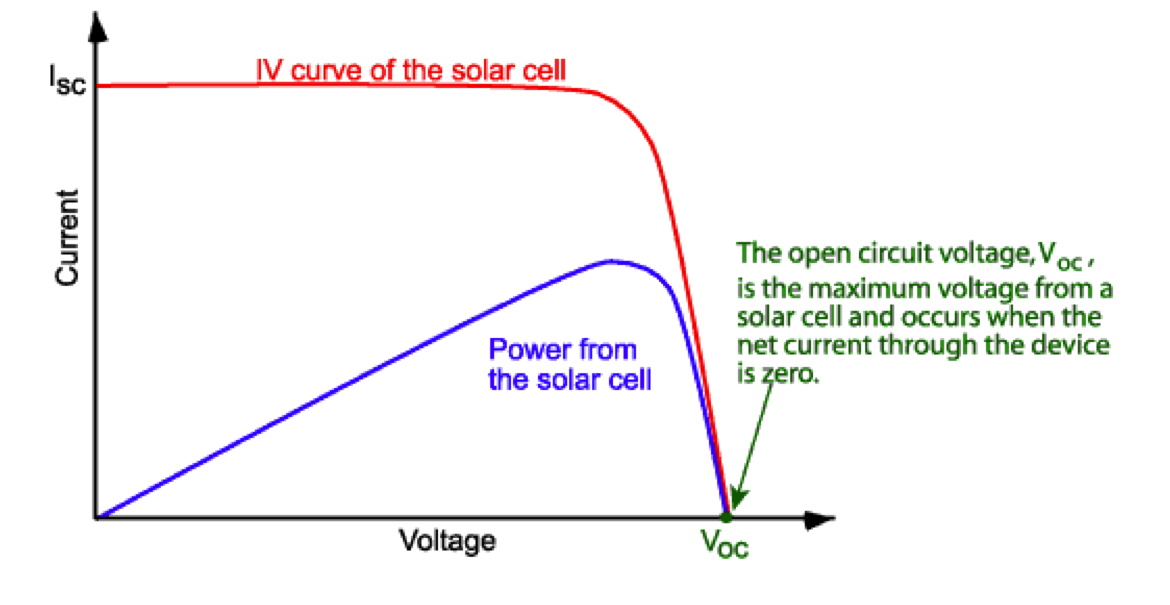
\includegraphics[width=0.65\textwidth]{figures/IV}
    \caption{The current-voltage (I-V) curve of a solar cell showing the open circuit voltage ($V_{OC}$). Figure taken from reference \citenum{PVeducation}.}
  \label{IV}
\end{figure}

When a cell consisting of a p-n junction is illuminated, a voltage develops across the terminals, i.e. between the p-type and n-type semiconductors. When the terminals of the solar cell are disconnected from any external circuit, or there is an infinite load resistance, this voltage is at a maximum and is called the open circuit voltage ($V_{OC}$) and no current is drawn from the solar cell. Conversely, if the terminals of the solar cell are connected together then there is no voltage as all of the electromotive force is used to extract charge-carriers. The maximum possible current is drawn, which is called the short circuit current ($I_{SC}$). For a solar cell to generate power, there must be both voltage and current generated, therefore when the cell is operating at either $V_{OC}$ or $I_{SC}$ the power output is zero. To generate power, a finite load resistance is added to the circuit so that some current is drawn from the solar cell and a voltage develops across the cell that is between 0 and $V_{OC}$ \cite{Nelson1}. There is a maximum operation point for the power output ($P_{MP}$) of a solar cell in terms of I and V, as shown in figure \ref{IV}. This can be defined in terms of $V_{OC}$ and $I_{SC}$ when used in conjunction with the fill factor (FF), which is a number less than one that describes the squareness of the I-V curve \cite{handbook} shown in figure \ref{IV} and is given by equation \ref{P_MP}. The current and voltage are determined by the load and illumination so the load can be tuned such that maximum power output is achieved, but the value of $V_{OC}$ places a limit on the power output of the cell \cite{Nelson1}.

\begin{equation} \label{P_MP}
P_{MP} = FFV_{OC}I_{SC}
\end{equation}

\begin{equation} \label{efficiency}
\eta = \frac{P_{MP}}{P_{in}} = \frac{FFV_{OC}I_{SC}}{P_{in}}
\end{equation}

The power conversion efficiency (PCE), $\eta$, of a solar cell is the ratio of power output from the solar cell to the power input from the Sun. This is shown in equation \ref{efficiency}, where $P_{MP}$ has been taken from equation \ref{P_MP}.
For an efficient solar cell, it is desirable to have a high $I_{SC}$, a high $V_{OC}$ and a FF that is as close to 1 as possible \cite{handbook}. CZTS solar cells are known to be hampered by low $V_{OC}$ relative to the band gap of the material \cite{SS}. Whereas in ferroelectric PV materials, photovoltages orders of magnitude larger than the band gap have been measured (a phenomena referred to as the anomalous photovoltaic effect), but very low photocurrent output is a big challenge for these devices \cite{FE_PV_rev1}.\\

**Add figure and description of basic PV device + show basic simplified band diagram (later compare to real band structure, e.g. of Si**\\

A solar cell device consists of... (see Mirjana's thesis)

\subsection{Key Properties \& Experimental Measurements to Assess Materials for Use in Solar Cell Devices}\label{PV_properties}
\begin{itemize}
\item PL
\item band gap
\item absorption coefficient
\item effective mass
\item dielectric function (screening of defects):   Why dielectric function is important - lower dielectric const in CZTS suggests electrostatic potential fluctuation is long ranged, material will be less `defect tolerant' - Look for textbook source!
\end{itemize}

\subsection{Current Commercial Solar Cell Technologies \& Limitations}
It was first observed in 1839 by Edmond Becquerel that sunlight could be used to generate electricity. Becquerel discovered that if  silver chloride was placed in an acidic solution, connected to platinum electrodes and exposed to sunlight, an electric current flowed. However the effect was small and poorly understood before Albert Einstein's discovery of the photoelectric effect and explanation of the phenomena by the quantum nature of light in 1904 \cite{PV_history1}. Even then, it was not until the development of semiconductor technology during the silicon revolution of the 1950's that solar cells were fabricated which were able to generate significant amounts of electricity. The first silicon solar cell was created in 1954 in the Bell Laboratories with cells achieving efficiencies of 6\%. 
Originally solar cells were developed for terrestrial energy generation, such as the 108 solar cells used to supply energy to the Vanguard satellite in 1958 \cite{PV_history1}. The first oil crisis in 1973 however highlighted the dependency of many economies on fossil fuels and the need to address the security of energy supply,  in particular for Japan and West Germany which had few of their own resources. As a consequence, solar cell research was no longer limited to only high-cost crystalline silicon devices for terrestrial applications, but also into creating cheaper, commercial, thin-film solar cell technologies using absorber materials such as amorphous silicon, cadmium telluride and copper indium diselenide  \cite{PV_history2}.\\

\begin{figure}[h!]
  \centering
    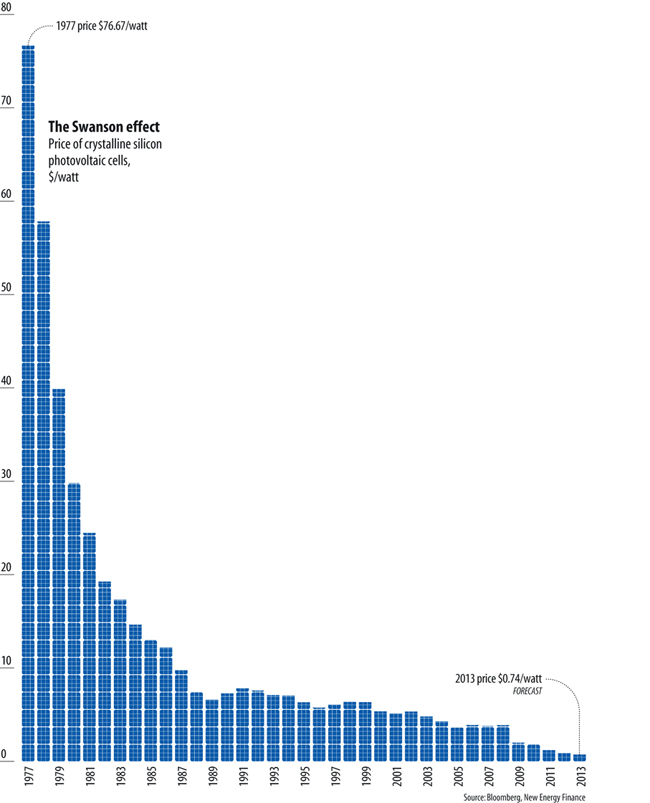
\includegraphics[width=0.9\textwidth]{figures/Si_cost.jpg}
    \caption{}
  \label{Si_cost}
\end{figure}

In spite of this, crystalline silicon is still the dominant solar cell technology with mono- and poly-crystalline silicon photovoltaic cells comprising up to 90\% of all the solar cells produced in 2008  \cite{Si_rev}. Silicon is the second most abundant element in the Earth's crust \cite{Si_abundance}, making it a plausible material to use in large-scale solar power generation. Over 60 years of development have seen device efficiencies increase from 6\% to 25\% for the highest quality research devices and 15-18\% for the more common industrial cells \cite{Si_rev}. As can be seen from figure \ref{SQ}, the best performing silicon devices are now very close to achieving conversion efficiencies close to their theoretical limit, as predicted by the Shockley-Quiesser detailed balance limit \cite{SQ_1961}. More dramatic however is the fall in manufacturing costs which have halved since 2008 and are more than a hundred times lower than they were in 1977, as shown in figure \ref{Si_cost}. This development was largely aided by progress in semiconductor technology driven by the silicon chip industry, with the solar industry benefiting from advances in silicon manufacturing processes and even making use of waste silicon produced that was not of a high enough grade for silicon chips \cite{PV_history1}. Although the development of silicon-based technologies has clearly revolutionized the modern computer, the optical properties of silicon do not make it ideal for use as a solar absorber material in a photovoltaic device and the technology is still not able to be cost-competitive with fossil-fuel power generation, as was shown in figure \ref{LCOE}.\\

The primary issue with silicon is that its band gap of 1.1 eV is indirect. The band structure of silicon is discussed in much more detail in section \ref{band_theory}, but the key consequence of this property is that silicon is therefore not a very strong absorber of sunlight (compared to for instance newer, thin-film technologies which are discussed later), resulting in a low optical absorption coefficient  compared to these newer technologies where both band gap and absorption coefficient were two of the key material properties for solar cells discussed in section \ref{PV_properties}. To absorb the same amount of sunlight with a silicon solar cell requires a thicker layer of the material than in thin-film technologies. Photovoltaic devices are very sensitive to defects and impurities. This point is discussed further in section \ref{defects_in_PV}, but the consequence for a thick layer of silicon is that very high quality, non-defective material is necessary to enable charge carrier collection before recombination occurs, which results in high manufacturing costs. The devices are made from flat sheets of crystalline or multicrystalline silicon called wafers that consist of very high quality silicon (99.999999\% pure) 
\cite{sus_book_5}.
The production processes of silicon wafers have been thoroughly optimised, but are still very energy-intensive, time-consuming and complex \cite{emerging_pv} and this is reflected by the position of this type of technology on the plot of efficiency versus cost shown in figure \ref{PV_generations}. Despite decades of development, commercialized silicon solar panels are still too expensive to compete with fossil-fuel based power sources \cite{FE_PV_rev1_5}. \\

The `holy grail' of research into new materials for photovoltaic devices would be to find materials that are strong absorbers of sunlight that could also be produced cost-effectively from materials that are abundant enough for large-scale fabrication of the devices. Then it could be possible for solar energy generation to be economically viable on a large enough scale to replace fossil fuels to meet global energy needs. Such a drive has resulted in the development of what are considered three generations of solar energy technology. These are shown in figure \ref{PV_generations}, where highly efficient crystalline silicon devices with high associated manufacturing costs are considered the first generation of solar cell technology.
Thin-film solar cell devices are typically referred to as second-generation technology. These devices make use of materials that are much more optically thick than silicon (i.e. stronger absorbers of sunlight with higher optical absorption coefficients), which require less material to absorb the same amount of sunlight. It is then less important for the material to be of as high-quality as in crystalline silicon devices, which enables the use of low-cost and low-energy fabrication methods \cite{emerging_pv}. 
In the case of thin-film CuInSe$_2$ devices, it has even been found that the `lower quality' poly-crystalline material has a higher performance than its single crystal counterpart \cite{CIS1_3, CIS1_4}. Theoretical studies of the electronic properties of the grain boundaries in CuInSe$_2$ have provided an explanation for this unusual observation based on beneficial band offsets at the grain boundaries \cite{CIS1, CIS2}. This effect is a special case for this particular material, but it embodies the general ideology of thin-film technology well - namely to produce materials able to convert sunlight into electricity as efficiently as possible with the simplest synthesis techniques possible.
However typically the efficiencies of second-generation solar cells are less than that of the best performing first-generation devices. Examples of commercial thin-film technologies include CIGS (Cu(In,Ga)(S,Se)$_2$) and CdTe and figure \ref{SQ} shows that the best performing Si devices have higher efficiencies, which are also much closer to their theoretical limit, than these second-generation, thin-film technologies.
Third-generation PV technology aims to make use of the low cost fabrication techniques of the second-generation devices but use multiple energy threshold devices to overcome the Shockley-Quiesser limit for a single band gap solar cell, such as in tandem solar cells where semiconductor p-n junctions of increasing band gap are placed on top of each other in order to capture more of the solar spectrum. Typically the more complicated device architecture of third-generation devices result in higher fabrication costs. Research efforts are therefore largely focused on reducing the fabrication cost of multi-junction devices \cite{3rd_gen}.\\

Current mainstream solar cell technologies, such as first-generation Si wafers and second-generation thin-film CdTe and CIGS solar cells, would not be able to provide solar electricity at the terawatt scale due to the scarcity of Te and In and the relatively long energy payback time for crystalline Si due to the cost and energy intensive fabrication of Si wafers \cite{CZTS_vs_MAPI}. In order to significantly increase the contribution of solar power to global power consumption, it is therefore necessary to develop economically viable earth-abundant materials for sustainable PV electricity generation. Furthermore, there must be a considerable technological breakthroughs that would enable low-cost manufacturing of highly efficient devices with enough of a cost benefit to outweigh the initial cost outlay in optimizing the manufacturing process of the whole device as has been done for silicon over the past 60 years. For this purpose, there is a drive for solar absorber materials with more optimal properties, such as a direct and sunlight matched band gap (as in thin-film technologies such as CdTe and CIGS), but also for materials that are composed of only earth-abundant components. 


\begin{figure}[h!]
  \centering
    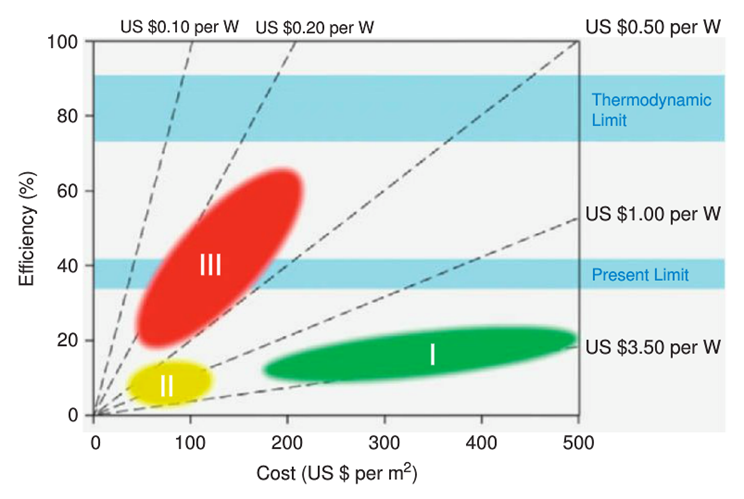
\includegraphics[width=0.75\textwidth]{figures/PV_generations.png}
    \caption{Efficiency and cost projections for first-, second- and third-generation photovoltaic technologies, which are comprised of silicon wafer, thin-film and advanced thin-film technology respectively. Figure 
 taken from reference \citenum{sus_book}.}
  \label{PV_generations}
\end{figure}

\begin{figure}[h!]
  \centering
    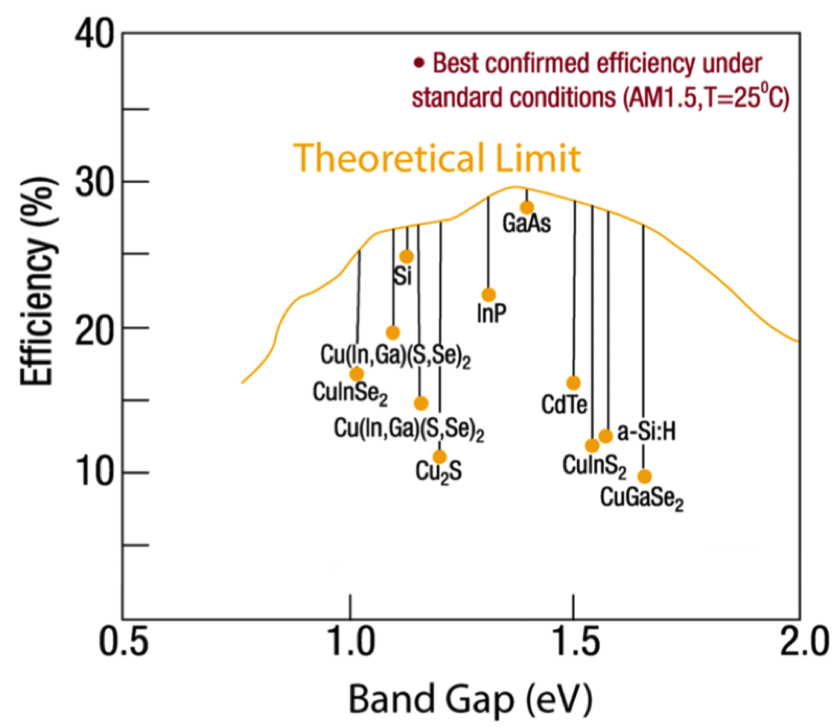
\includegraphics[width=0.65\textwidth]{figures/SQ.png}
    \caption{The Shockley-Queisser detailed balance limit of efficiency of p-n junction solar cells \cite{SQ_1961}, showing the theoretical limit and current record efficiency for various photovoltaic technologies. Figure courtesy of LL Kazmerski (NREL).}
  \label{SQ}
\end{figure}

\begin{figure}[h!]
  \centering
    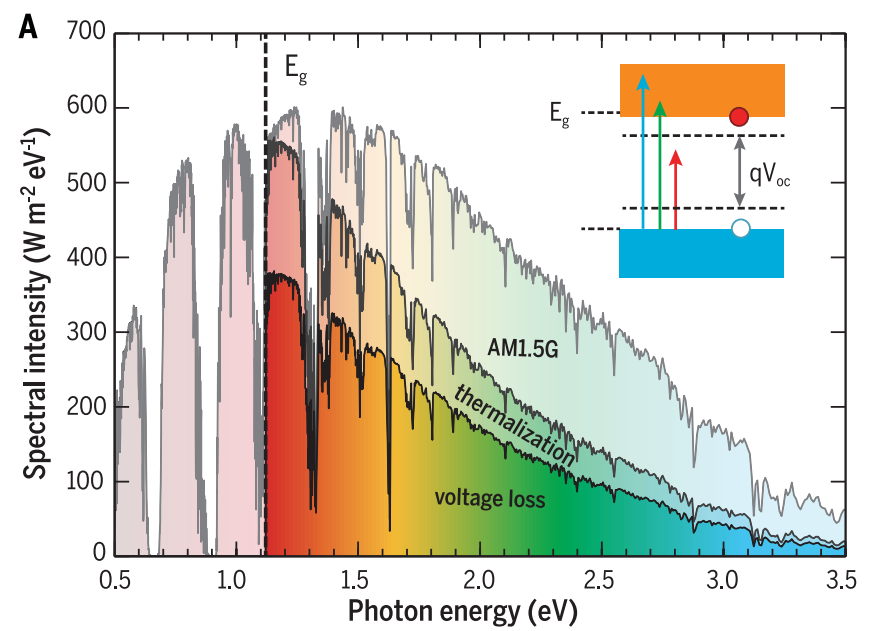
\includegraphics[width=0.95\textwidth]{figures/solar_spectrum2.png}
    \caption{Standard solar spectrum for radiation at the top of the atmosphere. Figure taken from reference \citenum{spectrum2}.}
  \label{solar_spectrum}
\end{figure}



\section{The Role of Computational Modelling in Material Design}
See DFT in materials science paper\\
Prediction of properties and insight for experimentalists + material screening\\

There are two main contributions that computational simulations could make towards the technological breakthroughs needed for the development of photovoltaic devices for economically-viable, large-scale solar energy generation. Firstly by predicting properties and screening for certain desirable properties for a solar absorber material, such as an optimal band gap and high carrier mobility, materials simulations are able to aid in the discovery of new materials for use in photovoltaic devices. Secondly, material simulations are able to provide valuable insight to improve understanding of known photovoltaic materials to enable the synthesis of better performing devices. So far in this study we have aimed to make both of these contributions to the field. Firstly, we perform simulations to understand the performance bottlenecks in the candidate earth-abundant, non-toxic solar absorber material \CZTS (CZTS) and we also study the optical properties of three candidate photovoltaic materials which have so far received little attention as solar materials but could be another possible route for high-performance photovoltaic devices for cost-effective solar energy generation.



\section{Overview of this Study}

\subsection{Promising Candidates for Solar Absorber Materials}
As already discussed, to make solar energy generation on a large scale economically viable, it must be possible to make devices with an LCOE that is comparable to fossil-fuel resources, but the materials that make up the devices must also be sufficiently abundant such that there would be enough to make a substantial number of devices in the first place. For this reason there is a drive for photovoltaic materials that could be made using the lost-cost methods associated with second-generation technology, but containing only earth-abundant components. Gauging the abundance of a given material is not as trivial a process as looking at crustal abundance as supply, demand, geographical distribution and extraction must all be considered. However some conclusions can be drawn by comparing one particular material to another, for instance the competition with the display industry for indium compared to zinc... Furthermore, another conclusion which can be drawn is that knowledge of solar cell technologies made from various different materials opens up the possibility of utilizing multiple different materials to collectively contribute to the global solar power capacity to enable larger-scale power generation from this renewable, low-carbon resource. Additionally by studying various different materials, the scientific community could eventually discover or invent some that could have the best properties to enable low-cost synthesis of highly efficient devices to eventually significantly reduce the LCOE of solar power.\\

Presently, two of the most studied candidate earth-abundant thin-film solar cell materials include Cu$_2$ZnSnS$_4$ (CZTS) and methylammonium lead iodide (CH$_3$NH$_3$PbI$_3$ or MAPbI$_3$) \cite{CZTS_vs_MAPI}. The potential of CZTS for photovoltaic applications was realised in 1988 by Ito and Nakazawa \cite{first_CZTS}. The band gap of the material has been predicted \cite{CZTS_bandgap_theory} and measured \cite{CZTS_bandgap_exp} to be 1.5 eV, which corresponds to a theoretical conversion efficiency limit of 28\% as predicted by Shockley-Quiesser photon balance \cite{SQ_1961}. However, the current record device efficiency is 8.8\% \cite{CZTS_record} and it is believed that this figure must be increased to at least 15\% for the devices to be commercially viable \cite{SS}. PV devices composed of a CZTS absorber layer are hampered by low open circuit voltage (V$_{OC}$) \cite{SS}, which is believed to be due to the formation of secondary phases \cite{CZTS_phases} and defects \cite{CZTS_defects} in CZTS, although the exact origin of the low V$_{OC}$ remains unknown. The first component of this study is therefore an attempt to determine possible origins of this deficit in CZTS.\\

MAPbI$_3$ is an example of a hybrid halide perovskite solar cell material, which are regarded as a convergence of inorganic thin-film and dye-sensitised solar cells (DSSC's) \cite{Federico}. Research on such materials dates back to 1928 \cite{Jarv_7}. The efficiency of MAPbI$_3$ solar cells however has increased rapidly between 2009 and 2014 from 3.8\% for MAPbI$_3$-based DSSC's to 20.1\% for a planar MAPbI$_3$-based thin-film solar cells \cite{CZTS_vs_MAPI} and has therefore surpassed the record efficiency of both conventional DSSC's as well as the earth-abundant thin-film PV absorber material CZTS \cite{Federico}. The architecture of a typical photovoltaic device, such as that shown in figure (**??**), is dependent upon charge separation by variation in material composition, as in a p-n junction. However, in ferroelectric materials charge separation can also be achieved due to the intrinsic crystal field in a homogeneous material. The crystal polarity creates microscopic electric fields across domains, separating photogenerated excitons into free charges, and segregating the transport of the free charges to reduce recombination rates \cite{keith}. Hybrid perovskites have been shown to exhibit spontaneous electric polarization \cite{Jarv}.
Therefore, one possible explanation for the high efficiency of MAPbI$_3$-based solar cells is enhanced separation of photoexcited electron and hole pairs, and hence reduced rate of electron-hole recombination, due to the presence of ferroelectric domains \cite{Jarv, Federico}. Although the stability of MAPbI$_3$-based solar cells has been identified as a big challenge for these devices, as CH$_3$NH$_3$PbI$_3$ is very sensitive to polar solvents such as water and so readily dissolves and decomposes into PbI$_2$ \cite{MAPI}. \\

A number of interesting photovoltaic phenomena have been observed in ferroelectric (FE) materials  such as the bulk photovoltaic effect (BPE) and the anomalous photovoltaic effect (APE) \cite{keith}. Ferroelectric materials usually have a high dielectric constant (which was mentioned earlier as an important parameter for a photovoltaic material) and they possess a spontaneous electric polarization that can be switched between two or more states using an electric field \cite{new_FE_PV_1}.
The BPE was first recorded in 1956 in BaTiO$_3$ \cite{keith_46}, where photovoltages were measured in un-doped single crystals \cite{keith}.
The BPE effect is distinctly different from the typical PV effect in semiconductor
p-n junctions as it is the polarization electric field that is the driving force for the photocurrent in FE-PV devices \cite{FE_PV_rev1}. The conventional PV effect is discussed further in section \ref{PV} and FE-PV phenomena are discussed further in section \ref{FE_PV_section}.
The APE was first observed in PbS films in 1946 \cite{keith_54} and has since been reported in polycrystalline CdTe, ZnTe, InP \cite{keith_55, keith_56, keith_57}, where photovoltages output along the polarization direction can be significantly larger than the band gap of the material \cite{FE_PV_rev1}, which is usually the limit for a semiconductor PV material \cite{keith}. 
The Shockley-Queisser limit, which prevents any single p-n junction solar cell from converting more than 33.7\% of the incident light into electricity has not been predicted to apply for these photovoltaic phenomena. An upper limit for the theoretical power conversion efficiency (PCE) from this photovoltaic mechanism seems to still be an open question \cite{new_FE_PV}, although an ultimate maximum efficiency of any single-band gap absorber of 44\% has been set by thermodynamic considerations \cite{SQ_1961}.
The identification and understanding of such phenomena may open up the possibility of more efficient PV devices constructed from a number of different photoferroelectric materials. However, most of the commonly used ferroelectric materials such as LiNbO$_3$ and BaTiO$_3$ have band gaps larger than 3 eV and can therefore only absorb sunlight in the UV range to convert into electricity, which accounts for only around 3.5\% of solar energy \cite{FE_PV_rev1}, which is illustrated in figure \ref{solar_spectrum}. The optimal range for the band gap in order to absorb the majority of the solar spectrum under typical radiation conditions is between 1.06 eV and 1.50 eV \cite{CZTS_book}. Research efforts have also gone into adjusting the optical absorption of ferroelectric materials without influencing the ferroelectric properties of the material through chemical doping or alloying \cite{FE_PV_rev1}. In Bi$_4$Ti$_3$O$_{12}$ (BiT) the optical band gap has been tuned in such a way, resulting in a decrease from 3.6 eV to 2.7 eV \cite{FE_PV_rev1_83}, although this is still considerably larger than the optimal range for a PV absorber material.\\

This then leads on to the second component of this study, which is an investigation of the optoelectronic properties of new candidate solar absorber materials that may also exhibit ferroelectricity, but have band gaps within the optimal range for the absorption of sunlight. In theory, these materials may exhibit the exceptionally high performance of MAPbI$_3$-based solar cells (ideally without the instability issues suffered by MAPbI$_3$) or enable the possibility of exploiting other novel photovoltaic phenomena such as the anomalous and bulk photovoltaic effects to overcome the Shockley-Quiesser efficiency limit without the need for such complicated device architectures as in third-generation tandem solar cells. Although the difference between the Shockley-Quiesser limit and the ultimate thermodynamic limit of a solar material is not enormous, it is also possible that ferroelectric materials have properties that enable more efficient devices to be made more easily, such as good screening of the effect of defects due to a high dielectric constant or enhanced electron-hole separation from ferroelectric domains resulting in reduced recombination and a higher performance solar cell with `low quality' defective and nanostructured materials. Such technologies could provide one possible route for the technological breakthrough that could enable economically-viable, large-scale solar energy generation.

\subsection{Investigating Possible Bottlenecks in the Performance of CZTS (\CZTS) Devices}

Mention kesterite as CZTS and CZTSe, combination of both gives highest performance but current study limited to just CZTS.

\begin{figure}[h!]
  \centering
    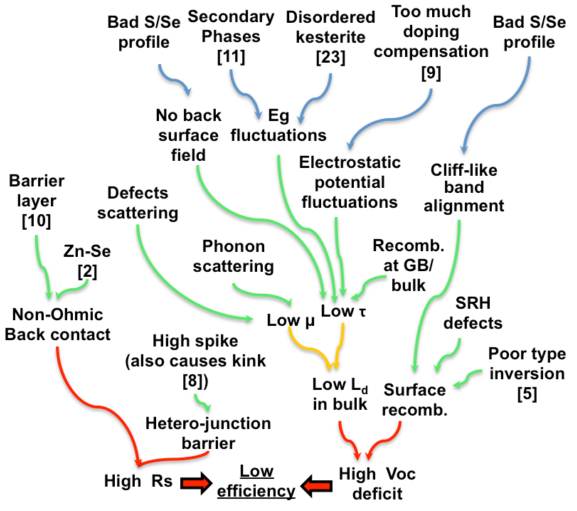
\includegraphics[width=0.75\textwidth]{figures/kesterite_bottlenecks.png}
    \caption{Figure take from \citenum{CZTS_scale_up}.}
  \label{kesterite_bottlenecks}
\end{figure}

Voc deficit + PL spectra of CZTS + disorder as a bottleneck --> essentially deciphering the PL spectra!
 
Photoluminescence (PL) spectra is discussed much more thoroughly in section \ref{PL_section}, but the key point for our study is that the PL spectra of CZTS differs considerably from the ideal case
(compare PL spectra of high quality Si, CdTe and CIGS?)

Although ultimately the aim is to make thin-film devices from CZTS, for the purposes of our study where we are currently simulating disorder in bulk CZTS, measurements performed on single crystals will be the most directly relatable to our findings as our model will not include additional spectra for recombination transitions and grain boundaries.

Other disorder studies providing evidence for Cu, Zn disorder: neutron, near-resonant Raman, etc. (see old report plan)

See Kosyak paper, top of pg 2 for discussion of why defect theory is important for CZTS because of limited exptl data whilst in early stages of development.

Ultimate aim of study is to unpick/ decipher the PL spectra of CZTS to determine sources of efficiency loss to guide experiment. There are a number of possible explanations for the PL spectra such as mid gap states (which would give rise to additional sharp optical transitions and energies below the band gap of the material),  band gap broadening due to intrinsic lattice vibrations but also to disorder and band tailing due to various types of disorder.

We first study band tailing from metal disorder in CZTS. We also re-investigate the formation of S vacancies when accounting for S being in the gas state, using a full S chemical potential as $V_S$ has been predicted to give a mid gap energy state, but calculations consider S in only the solid state have predicted a high defect formation energy and therefore the presence of this type of defect unlikely. This may not be the case when accounting for S being in the gaseous state during the synthesis of CZTS.
We then go on to attempt to determine how much of the band gap broadening observed in CZTS (*REF PVTEAM PAPER*) is due to disorder by calculating the intrinsic (and inevitable!) contribution from the lattice expansion of perfect CZTS at finite temperatures, and subtracting this from the experimentally measured broadening.
 
But there are a number of further investigations (see further work section): larger systems, domains, band gap fluc + compensating defects for off-stoichiometric systems


\subsection{Predicting and Assessing the Properties of New Candidate Solar Absorber Materials}
Ferroelectric materials in PV devices\\
Screening criteria\\
Properties of interest for PV (discussed above) which we aim to predict for these materials + known exptl and theoretical values from the literature (see MRes2 report and new bournonite paper)



